\documentclass[twoside,bibtotoc,BCOR=9mm]{scrreprt}
\usepackage[utf8]{inputenc}

%\usepackage{palatino}
\usepackage[sc,osf]{mathpazo}
\usepackage{microtype}

\usepackage[german,english]{babel}
\usepackage{amsmath}
\usepackage{natbib}
\usepackage{tabularx} 
\usepackage{setspace}
\usepackage{color}
\usepackage{tuebingerspruechle-utf8}
\usepackage{graphicx}
\usepackage{rotating}
\usepackage{listings}
\usepackage{multicol}
\usepackage{acronym}
\usepackage{avm}
\usepackage[pdftex,breaklinks=true]{hyperref}
\usepackage{gb4e}
\usepackage{float}
\usepackage[T1]{fontenc}
% \usepackage{verbatim}

\hypersetup{pdftitle={Title Goes Here}}
\hypersetup{pdfauthor={Author Goes here}}
\hypersetup{pdfsubject={}}
\hypersetup{pdfkeywords={}}

\definecolor{UniBlue}{rgb}{0,0.24,0.5}
\definecolor{FurtherResearchColor}{rgb}{0.5,0,0}
% KOMA script fonts
\setkomafont{title}{\bfseries\color{UniBlue}}
\setkomafont{sectioning}{\normalfont}
\addtokomafont{sectioning}{\color{UniBlue}}

\avmfont{\sc}
\avmoptions{sorted,active}
\avmvalfont{\rm}
\avmsortfont{\scriptsize\it}


\bibpunct{(}{)}{;}{a}{,}{,}
\setcounter{secnumdepth}{5}
%\setcounter{tocdepth}{3}

% set spacing for easier reading (and more pages...)
\onehalfspacing

\newcommand{\todo}[1]{\textsc{\textbf{\color{red}TODO:} #1}}
\newcommand{\furtherresearch}[1]{\small\color{FurtherResearchColor}\textsc{Further
Research:} #1}

\newcommand{\boxnum}[1]{
{\fbox{\footnotesize {#1}}}
}

% some formatting commands
\newcommand{\classname}[1]{{\tt {#1}}}
\newcommand{\methodname}[1]{{\tt {#1}}}
\newcommand{\ifacename}[1]{{\tt\itshape {#1}}}
\newcommand{\packagename}[1]{{\sf\itshape {#1}}}
\newcommand{\code}[1]{{\tt {#1}}}

% new lst environment for code snippets
\lstnewenvironment{plainsnippet}
{
  \lstset{
    basicstyle=\footnotesize\tt,
    frameround=ffff,
    frame=trbl,
    xleftmargin=1cm,
    xrightmargin=1cm,
    %aboveskip=.4cm,
    %belowskip=.4cm,
    aboveskip=.5cm,
    belowskip=.5cm,
    extendedchars=true,
    inputencoding=latin1
 }
}
{}


\begin{document}
\bibliographystyle{plainnat}
% \bibliographystyle{acl}

% TITLE --------------------------------------------------------------------
\titlehead{\begin{multicols}{2}
\begin{flushleft}
{\Large Universität Tübingen\\}
Seminar für Sprachwissenschaft\\
Wilhelmstraße 19\\
72074 Tübingen\\
\end{flushleft}
\begin{flushright}

\includegraphics[scale=0.353]{uni-logo.pdf}
\end{flushright}
\end{multicols}}
\subject{M.A. Thesis in Computational Linguistics}
\title{Android App Development for Language Learning: Combining input and interaction in learning German through song lyrics}
\author{Alina Baranova\\
  {\small \texttt{alina.baranova@student.uni-tuebingen.de}}}
\publishers{
\begin{tabular}{ll}
First Examiner and Supervisor: & Prof. Dr. Detmar Meurers\\
Second Examiner: & Second, PhD \\
\end{tabular}}
\date{}  
\maketitle
\SpruechleAufsagen{Alina Baranova}
\clearpage

{\centering \Large \color{UniBlue} Abstract\\[.5cm]}
ENGLISH ABSTRACT HERE
\clearpage
\selectlanguage{german}
{\centering \Large \color{UniBlue} Zusammenfassung\\[.5cm]}
GERMAN ABSTRACT HERE
\selectlanguage{english}

\tableofcontents
% \pagebreak

{
\singlespacing
\begingroup
\let\chapter=\section
\let\addchap=\addsec
% \listoftables
% \listoffigures
\endgroup
}


\chapter{Introduction}

Icons made by <a href="https://www.flaticon.com/authors/freepik" title="Freepik">Freepik</a> from <a href="https://www.flaticon.com/" title="Flaticon"> www.flaticon.com</a>

<div>Icons made by <a href="https://www.flaticon.com/authors/pixel-perfect" title="Pixel perfect">Pixel perfect</a> from <a href="https://www.flaticon.com/" title="Flaticon">www.flaticon.com</a></div>

\chapter{Related Work}
\label{sec:related-work}

This section is devoted to the overview of the existing systems that offer the user a possibility to learn languages through song lyrics. Only websites and applications that involve exercises based on songs texts are examined. Thus, collections of song lyrics and their translations are not taken into account.

The following systems are examined: \textit{LyricsTraining}\footnote{\url{https://lyricstraining.com}}, \textit{FluentU}\footnote{\url{https://www.fluentu.com}}, \textit{LyricsGaps}\footnote{\url{https://www.lyricsgaps.com}}, and \textit{Language Zen}\footnote{\url{https://www.languagezen.com/en}}. All the four systems have a web version and a mobile version. Although the creators usually invest in one of the versions more, features of both web and mobile versions are discussed.

Different aspects of systems are analyzed: possible modes of discovering lyrics, type and structure of exercises for memorizing new words, language levels that the system offers, translation of separate words and whole lyrics into English. Moreover, the number of languages supported by systems and features not connected to song lyrics are mentioned. The systems that have more popular Android apps are highlighted first.

\section{LyricsTraining}

According to the Google Play\footnote{\url{https://play.google.com/store}}, an official app store for the Android operation system, the mobile version of \textit{LyricsTraining} is the most popular among the four systems mentioned here, and has more than 500,000 downloads\footnote{Accessed: June 28, 2019}. The system is solely developed for using music lyrics in language learning. When clicking on each song, the user can choose one of the two modes: karaoke mode and game mode. In game mode, a level should be selected: beginner, intermediate, advanced or expert. The more difficult the level is, the greater number of blanks in the text is. In web version, every song lacks either 10\%, 25\%, 50\% or 100\% of the words. In mobile version, number of words transformed into questions differs from song to song, but in expert level the user has to fill in all words in the lyrics, as in the web version. Such task is very unlikely to be accomplished, regardless of the language level of the user. Moreover, it hinders one of the main goals of learning vocabulary through song lyrics --- learning new words in context. Therefore, for expert level, it would be reasonable to decrease the number of words that are transformed into questions.

In all the other three levels in mobile version, the number of words extracted from the text seems to be dependent on the pace of the song. It is more comfortable than filling in 10\%, 25\% or 50\% of song lyrics, as in some very fast songs it might be too hard for the user to accomplish a higher level, which can possibly lead to his/her frustration.

Type of exercises in a mobile and in a web version are different: it is multiple choice questions and fill-in-the-blank questions accordingly. For every multiple choice question in the mobile version of \textit{LyricsTraining}, three distractors are available, all of them the words from the other blanks in the song. On the one hand, it makes it too easy for the user to guess the word while hearing it, as the distractors are not especially chosen to sound similarly to the right answer. On the other hand, the user is less stressed, as he/she needs less time to make a decision about the next word, because the three out of four options from the previous question stay the same in the next one. Apart from that, it is programmatically more simple to use words from other blanks as distractors, as there is no need in an external source for obtaining them. Moreover, due to the fact that the distractors need not be picked beforehand, this allows random generation of blank spaces, which is implemented in \textit{LyricsTraining}. 

Fill-in-the-blank questions in the web version are considerably harder than multiple choice questions, especially when the singer uses slang, and the song is rather fast. In a combination with choosing to fill 50\% of the lyrics, it might provoke user's dissatisfaction with his/her result. When comparing the game mode in the web version and in the mobile version, the latter appears to be more sensible and thought-out.

In the game mode, both in the web and in the mobile version, a music video is synchronized with the lyrics, and a certain time limit is implemented --- the user should choose the option or type in the answer as soon as the line was sung. If the user did not know the right word the first time, there is a possibility to hear the line again or to see the right word and go to the next blank space.

Apart from the game mode, the user can choose a karaoke mode. In this mode, as in the game mode, a music video is synchronized with the lyrics, so that the line sung at the moment is highlighted. Unlike in the game mode, however, user does not have to fill in any words and can switch the song backward and forward. This mode is suitable for either hearing the song for the first time, before the game mode, or afterwards, so that the user can memorize the new words he/she encountered.

Unlike some other systems, \textit{LyricsTraining} does not allow clicking on words in the song to obtain their translations and does not offer translations of the whole lyrics either. However, there is a section \textit{My vocabulary }in the mobile version, where separate words can be translated into 58 other languages through the Microsoft Translator.

Even though only the German version of the \textit{LyricsTraining} was tested, the system is offered in twelve other languages, among them e.g. Japanese and Turkish.

\section{FluentU}

The system with the second popular Android app is \textit{FluentU}, which has more than 100,000 downloads\footnote{Accessed: June 28, 2019}, according to Google Play. Music videos is only one of the resources for language learning the system offers. For the first two levels, Beginner 1 and Beginner 2, audios on grammar topics are available. For all the levels, videos on different topics (e.g. \textit{Arts and Entertainment} and \textit{Science and Tech}) are accessible. The videos have different formats, too, such as \textit{Mini-movies} or \textit{Talks/Speeches} --- and among them, \textit{Music videos}.

There are three possible ways one can work with a music video. First, there is a dialogue mode, where the user can read through song lyrics and its line-by-line translation into English. The vocabulary mode contains the words that are taken from the song text and are supposed to be learnt by the user through the quiz. The last mode is playing the video. In this mode, lyrics and videos are synchronized, and the user can go backward and forward. As \textit{FluentU} is one of the systems that allow translating separate words and phrases in the song text, the user can click on any word of the line that is being sung at the moment and acquire the word's translation, while the video is automatically paused. The translations are very detailed, they include the part of speech, some specific characteristics for this part of speech, such as gender for nouns, an audio with a native speaker pronouncing the word and general example sentences. In the web version, the translations are supplemented with example sentences from the song and a suitable picture. 

In order to train the vocabulary from the song, the user can do a quiz. There are three types of the exercises: multiple choice questions, fill-in-the-blank questions and ordering. Multiple choice questions include, for example, choosing a right translation of a sentence from English into German. An example of a fill-in-the blank questions would be selecting the right word to complete the sentence. Finally, ordering is concerned with putting the words int the right order to get a line from the song. The quiz is done after watching the video, and there is no time limit for answering the questions.

All the music videos are assigned levels. There are six levels in total: Beginner 1 and 2, Intermediate 1 and 2, Advanced 1 and 2. The more difficult the level, the less music videos is available --- thus, Advanced 1 and Advanced 2 have only two and one music videos accordingly. There are two ways of solving this problem: either more videos can be added or each music video could be adapted for other levels. There are forty videos in total, and there are some learner-specific songs among them as well --- for instance, \textit{The Umlaut Song!} or \textit{Numbers 1-10 Singalong}. This kind of songs are probably not that interesting for an average music lover, even though they might be helpful in memorizing the vocabulary.

Apart from German, nine more languages are implemented, including, for example, Korean and Russian.

Compared to \textit{LyricsTraining}, \textit{FluentU} uses a more complicated quiz-format, which can be more helpful for memorizing the vocabulary. However, \textit{LyricsTraining} offers interactive learning, which \textit{FluentU} lacks. This way of learning might be more entertaining for the user. A very small number of music videos is available in \textit{FluentU}, but there are some other activities for learning implemented in the system, so it cannot be considered a big disadvantage.  
The big advantage of \textit{FluentU}, on the other hand, is the possibility to translate words and phrases while listening to the song, as well as an access to translations of the whole lyrics, which is not found in \textit{LyricsTraining}.

\section{Language Zen}

The third most popular Android app belongs to \textit{Language Zen} and has more than 10,000 downloads\footnote{Accessed: June 28, 2019}, according to Google Play. As \textit{FluentU}, \textit{Language Zen} offers other ways to learn languages: the user can choose the courses mode, which contains phrases and vocabulary split into topics, or start learning the most frequent words. 

In contrast to other systems, \textit{FluentU} only offers two languages to learn. In web version, it is only Spanish for English speakers, and in the mobile version, there is also a possibility to learn English for Portuguese speakers. The creators of the system are planning to implement more languages in the future. Only the course in Spanish for English speakers was analyzed. 

When the user chooses a song, he/she can either select the play mode or the learn mode. In the play mode, lyrics and audios are synchronized, and the user can play the song forward and backward, as in the other systems discussed so far. \textit{Language Zen} also offers translations of individual words when clicking on them. Apart from that, every line is followed by its translation. Translations of some individual words (e.g. \textit{se}) are complemented with short grammar notes that explain their usage (e.g. \textit{Passive ``se''}). In the web version, word forms are also morphologically analyzed --- for example, a verb is assigned number, person and tense in present tense, and a noun --- number and gender.

The learn mode offers a quiz with multiple choice and fill-in-the-blank questions. The user is asked to translate words and phrases from Spanish to English and vice versa. An interesting feature of the system is the way things that the user learnt or attempted to learn before are included in the quiz even if a song which is new for the user is chosen. There is no time limit for answering questions.

There are many levels of Spanish the user can choose from: beginner, beginner plus, intermediate, intermediate plus, advanced, advanced plus and fluent. There is also a near native level, which is only present in the web version. However, to take any level higher than beginner, the user should pass an assessment test. Beginner level offers only fourteen songs; other levels were not examined. 

\section{LyricsGaps}

The system that has the least popular Android app among the four systems examined in this section is \textit{LyricsGaps}. According to Google Play, there are more than 500 downloads\footnote{Accessed: June 28, 2019} of this app. It is nevertheless important to point out that the web version of the system is much more developed than its mobile version. 

As \textit{LyricsTraining}, \textit{LyricsGaps} is fully devoted to learning languages through song lyrics. Exercise mode is shared by both the mobile and the web version. The web version, however, also offers a karaoke mode and a word-to-word mode. The karaoke mode displays the whole text, and, unlike in other systems, the song and its lyrics are not synchronized, so the line sung at the moment is not highlighted. The word-to-word mode is rather strange: it is supposed that the user has to click on every word of the song while playing the video.

In the web version, exercise  mode includes texts with multiple choice and fill-in-the-blank gaps. The type of questions depends on the level chosen by the user. Multiple choice questions offer too many distractors --- usually, all the words from other blank spaces are used for that. Using only a few distractors, as in \textit{LyricsTraining}, would be more benefiting for users in this case, as it will not confuse them that much. In the mobile version, only three distractors are used. However, every line has a blank space that should be filled with one of the four possible options, which results in more gaps than in the web version.

In some sense, one can speak about time limit in the mobile version, as the user has to type in an answer fast enough to follow the song. If he/she does not type the answer in time, the song does not stop, as, for instance, in \textit{LyricsTraining}. This kind of design might have a negative impact on the results of the user and their satisfaction with the system. In the web version, there is no time limit, and the user can listen to the song as many times as he/she would like.

As has been mentioned before, in the web version the user has the opportunity to choose a level of the exercise: beginner, intermediate or expert. Beginner level exercises include multiple choice questions, and the other two levels offer questions of fill-in-the-blank type, which are objectively harder for the user. No correlation between the level and the number of gaps in the text is found, although there are on average more gaps in songs with longer texts\footnote{Five songs from different artists were analyzed}. 

Even though the system does not provide translations of whole lyrics, the user can acquire translations of separate words by clicking on them. If the word form is different from its lemma, the translation of the word form will be shown --- for example, \textit{gab} would be translated into English as \textit{gave}. Apart from English, translations into nineteen other languages are possible. Unfortunately, translation of words is only available in the web version of the system.

\textit{LyricsGaps} is accustomed to twenty languages, not including German. Compared to three other systems, it is the greatest number of languages offered. Among popular languages, such as French and Chinese, more exotic ones are offered --- for instance, Indonesian or Catalan.

To sum up, there are two systems that offer exercises while listening to a song, and two systems where exercises should be done after listening. A system can either contain different songs for different levels or adapt each song to several levels. In most of the systems, songs are synchronized with their lyrics, and the user is able to click backward and forward buttons to control the song. The maximum number of languages offered is twenty-one, and the least is two. In three out of four systems, translations of separate words are possible. Two of these systems also contain translations of whole lyrics.

\chapter{Song Selection}
\label{sec:selection}

For creating an app for learning German grammar through songs, a set of songs needed to be sampled. Consulting German second language, or L2 learners allowed to address the issue objectively, independent of the author's own musical preferences, and receive a number of artists belonging to various genres.

Google Forms\footnote{\url{https://docs.google.com/forms/}}, one of the platforms for online questionnaires, was used for getting information about favorite German artists of language learners. Students whose native language is not German were asked to name three artists or bands whose songs they would like to see in an application for learning German. Every person taking part in the questionnaire was asked to write down three names of artists and choose an appropriate genre for each of them. There were ten options to choose a genre from: pop, rock, dance/electronic/house, soundtracks, hip-hop/rap/trap, singer/songwriter, classical, R\&B, soul/blues, metal. The set of genres was taken from Music Consumer Insight Report conducted in 2018 by ifpi [CITE]. To make a list of the ten most popular genres for this report, 19,000 participants from eighteen countries were surveyed. As in the survey for the most popular music genres, the data received from the questionnaire was based on participants' own definitions of genres.

In total, twenty-three people filled the form, which resulted in a sample of fifty-five unique artists.

As the app is dependent on YouTube [CITE???] for getting audio-tracks for songs, the songs were chosen based on this video-sharing platform. It was decided to take a random number of songs --- three --- by every artist. For choosing songs, videos by an artist were sorted by the greatest number of view counts. Moreover, only songs with official videos of the artist were chosen. Official lyrics videos --- as, for example, \textit{In Deiner Kleinen Welt} by Philipp Dittberner --- were also taken into account. Sometimes, however, it was unclear which video can be counted as official, as an artist or band did not have an official YouTube channel --- for instance, in case of the band \textit{Ja, Panik}. In such cases, the videos that looked like video-clips were chosen. Another important criteria was choosing songs by an artist or band alone, without other musicians featuring in the videos. Nevertheless, this rule also led to an exception, as most of the songs by Audio88 are made in a collaboration with a rapper Yassin. On this stage of sampling a song set, an artist or a band were excluded if they did not have official videos or at least videos that look like video-clips.

Downloading lyrics manually from the Internet would take a considerable amount of time, that is why ways of doing it automatically have been surveyed. According to the website of Genius\footnote{\url{https://genius.com/}}, it contains ``over 25 million songs, albums, artists, and annotations'', while providing an API that can be used for downloading song lyrics. Apart from that, LyricsGenius\footnote{\url{https://github.com/johnwmillr/LyricsGenius}} --- a Python client for the API --- is available. The following code allows downloading lyrics using song name and artist name:

\begin{lstlisting}[language=Python, caption={Downloading song lyrics}, label={lst:genius}]
    import lyricsgenius
    
    genius = lyricsgenius.Genius(CLIENT_ACCESS_TOKEN_HERE)
    song = genius.search_song(SONG_NAME, ARTIST_NAME)
    
    print(song.lyrics)
\end{lstlisting}

However, not all songs that have videos on YouTube also have lyrics on Genius.com. To avoid such songs, it was checked if the most popular song on YouTube by the artist is provided with lyrics on the website. If this was not the case, songs of the artist were not included in the sample. 

All in all, forty-four out of fifty-five artists acquired with the questionnaire were left, resulting in 131 songs for the sample. Only one song by one of the forty-four artists --- \textit{Am ersten Sonntag nach dem Weltuntergang} by Element of Crime --- was not featured on Genius. That shows that the strategy to predict which artists have song lyrics on the website by checking the most popular song is rather accurate.

After acquiring names of songs and their artists, lyrics were automatically downloaded with the code similar to Listing \ref{lst:genius}. The only strange result was produced by downloading song \textit{Auf uns} by Andreas Bourani --- instead of the song text, one would get a list of songs by different artists. Due to this problem, lyrics for this song were manually copied from the website. 

When all the texts were downloaded, some parts of texts which would hinder synchronization of lyrics with audio have been deleted e.g. ``[Strophe II]:'' or text in brackets in ``Ja ja, ich weiß [10x]''. Due to examples of the second type, is very probable that at the stage of synchronizing song text with audio some lines will need to be inserted.

\chapter{Lyrics-to-Audio Alignment}
\label{sec:alignment}

\section{Automatic Alignment}

Automatic lyrics-to-audio alignment is a problem that might seem similar to the problem of automatic speech recognition. However, some characteristics of singing voice are very different from the ones of speech, which prevents the usage of speech recognizer for performing the alignment.

Firstly, acoustic characteristics, such as pitch and loudness, tend to fluctuate much more in singing than in speech. Secondly, sounds in singing, especially vowels, tend to be prolonged or shortened, which results in larger variation of sound duration compared to speech \citep{Kruspe.2018}. The background music is the third difference between singing and speech. As the spectrum of singing voices gets affected by accompaniment sounds, it makes the process of lyrics-to-audio alignment more difficult \citep{Fujihara.2012}. For this reason, some studies prefer working with unaccompanied singing rather than with polyphonic music.

Some minor difficulties of recognizing or aligning singing voice also include lyrics-specific vocabulary, which differs from vocabulary used in spoken language \citep{Kruspe.2018}, and incomplete song texts, especially due to omitting interjections such as \textit{oh} or \textit{yeah} \citep{Fujihara.2012}.

As was briefly mentioned above, there are studies aiming at singing voice recognition e.g. \cite{Kruspe.2018} and \cite{Sasou.2005}, as well as the ones concentrating on lyrics-to-audio alignment. In this thesis, only works on alignment of singing voices to songs texts will be reviewed. There is also some research done on unaccompanied singing \citep{Loscos.1999, Sasou.2005, Gong.2015}. However, the task of lyrics-to-audio alignment in polyphonic music is more suitable for the future Android application, so studies on unaccompanied singing are left out in this evaluation.

The granularity of lyrics-to-audio synchronization can be different --- possible fragments of lyrics include phoneme \citep{Mauch.2012}, syllable \citep{Iskandar.2006}, word, phrase \citep{Fujihara.2006, Dzhambazov.2016}, line \citep{Wang.2008, Wong.2007, Mesaros.2008}, paragraph \citep{Lee.2008} and section \citep{Wang.2008}, which, depending on the interpretation, can correspond to paragraph-level alignment. Among the works that are analyzed in this section, synchronization on line level is chosen for the greatest number of studies. This granularity of synchronization is also the best option for the Android application that is being developed.

As could be expected, most authors choose songs in English to evaluate their approach. There are, however, singular studies that concentrate on other languages, such as Japanese \citep{Fujihara.2006, Fujihara.2008}, Cantonese \citep{Wong.2007} and Turkish \citep{Dzhambazov.2016}. To the best of my knowledge, no systems have been analyzed on songs in German.

It is unclear how many songs should be included in the test set to provide reliable results, but, except for one work where the system was tested on three songs only \citep{Iskandar.2006}, studies typically include from ten to twenty songs in their test set.

Metrics used to evaluate how successful a system performs the alignment task often differ from one study to another, which makes it difficult to compare results between various studies, especially if the granularity of synchronization is also different. Evaluation metrics include average displacement error \citep{Wang.2008, Lee.2008, Mesaros.2008}, average word error rate \citep{Iskandar.2006} and average accuracy \citep{Fujihara.2006, Fujihara.2008, Mauch.2012, Dzhambazov.2016}, with average accuracy being the most popular metric. Among systems evaluated with the accuracy metric, the best one achieves accuracy of 0.88 on a phoneme level \citep{Mauch.2012}. If one chooses average displacement error as an evaluation metric, the smallest error\footnote{A mean error of 7.34 and 9.03 seconds has been achieved in \cite{Kruspe.2018}, but it is hard to compare this result to other works due to their different granularity.} would be 0.58 seconds on a line level \citep{Wang.2008}. Both systems are tested on English songs.

Unfortunately, even though the two systems show rather impressive result, they are not publicly available. Moreover, the accuracy of synchronisation is crucial for the app, as it ensures interactive learning, and even an error of  half-a-minute would make a difference. Apart from that, if some of the methods used in the systems appear to be language-specific, the systems would also not be applicable for songs in German. In addition, not too many songs are included in the app initially. Due to these reasons, manual lyrics-to-audio alignment was preferred over automatic alignment.

\section{Manual Alignment}

There are several programs that support the process of manual lyrics-to-audio alignment.

\subsection{GNMIDI}

This program is only available for Microsoft Windows users, and offers a possibility to manually align half of the lyrics in its free version\footnote{Demo version of GNMIDI 3.17 was tested.}. The user pastes the text of the song as a whole and aligns the lines of the lyrics to the audio by pressing the \textit{Enter} key when a line is sung. In this way, a file of LRC format is created, where every line of the lyrics is assigned the time when it is sung (see Figure \ref{fig:lrcFormat}\footnote{Example taken from \url{https://en.wikipedia.org/wiki/LRC_(file_format)}}). In files of this format, the time is usually written as \textbf{[mm:ss.xx]}, where \textbf{mm} stands for minutes, \textbf{ss} --- for seconds, and \textbf{xx} --- for hundredths of seconds. 

\begin{figure}[H]
    \begin{verbatim} 
        [00:12.00]Line 1 lyrics
        [00:17.20]Line 2 lyrics
        [00:21.10]Line 3 lyrics
        ...
        [mm:ss.xx]last lyrics line  \end{verbatim}
    \caption{LRC Format}
    \label{fig:lrcFormat}
\end{figure}

When the user exports the resulting file from GNMIDI, however, no hundredths of seconds are saved in the file. The karaoke demonstration in the program (see Figure \ref{fig:karaokeDemo}) also relies on times without hundredths of seconds. 

\begin{figure}[H]
    \centering
    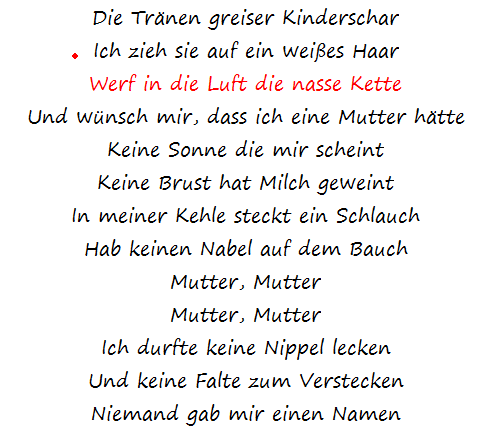
\includegraphics{../images/gnmidiScreenshot.png}
    \caption{GNMIDI Karaoke Demonstration (song \textit{Mutter} by Rammstein)}
    \label{fig:karaokeDemo}
\end{figure}

Apart from that, GNMIDI does not support UTF-8 format, which is important for lyrics in German.

\subsection{SYLT Editor}

SYLT Editor is a free software, and versions both for Microsoft Windows and Linux are available\footnote{SYLT Editor 1.1 was tested for this section.}. In contrast to GNMIDI, the program supports UTF-8 encoding. However, loading LRC-format file with lyrics has failed, so the song text had to be entered line by line. After the user assigned times to lines of the lyrics by pressing the \textit{Space} button when a line is sung, the text should be able to be exported to a file of LRC format. Unfortunately, exporting a file, as well as importing a file, was not possible due to an occurring error.

\subsection{Megalobiz: LRC Maker \& Generator Online}

LRC Maker \& Generator Online is a website\footnote{\url{https://www.megalobiz.com/lrc/maker}} where one can align lyrics to audio of the song after loading an MP3-file and pasting in the text of the song. When a line is sung, the user must click on this line for it to be assigned the time. The user can also check if he/she aligned the lines in a right way by playing the song again --- the lines of the lyrics will be highlighted according to assigned times. To save the file in LRC format, the user should press the button \textit{Save}, which results in a UTF-8 encoded file on his/her computer.

To sum up, LRC Maker \& Generator Online is the best choice for manual lyrics-to-audio aligning, as it saves the hundredths of seconds in time tags, in contrast to GNMIDI, and is able to export the resulting file, unlike SYLT Editor. Moreover, the website is completely free to use. The website was used for tagging song texts used in the Android app.
\chapter{Grammatical Questions}
\label{sec:grammar}

\section{Grammar Topics}

\section{Tools For Extracting Grammatical Constructions}

In order to extract chosen grammatical constructions from song texts, a suitable dependency parser is needed. Four dependency parsers trained on German texts are analyzed in this section: ParZu, spaCy, the Stanford Parser and the Mate tools parser.

\subsection{Dependency parsers}

ParZu \citep{Rico.2009} was trained on Europarl and includes the following components in its pipeline: sentence segmentation, tokenization, part-of-speech (POS) tagging, morphological analysis and the core component --- dependency parser, with a preprocessing step before and a postprocessing step after it. Remarkably, for all the tasks except dependency parsing, ready-made tools were chosen e.g. the punkt\_tokenizer from NTLK was used for tokenization, and clevertagger\footnote{\url{https://github.com/rsennrich/clevertagger}} --- for POS-tagging. The POS-tagger uses the Stuttgart-Tübingen Tag Set (STTS). The dependency analysis is represented in the CoNNL dependency format and includes an index, a lemma, a POS-tag, a language-specific POS-tag, morphological features, a head and a dependency relation for every token. The three other parsers use a similar set of features.

spaCy\footnote{\url{https://spacy.io/}} was trained on TIGER Corpus and WikiNER dataset, and it provides two models for parsing German texts: \textit{de\_core\_news\_sm} (the small model) and \textit{de\_core\_news\_md} (the medium model), with \textit{de\_core\_news\_md} performing with a higher accuracy. Linguistic features supported by spaCy include sentence segmentation, tokenization, POS-tagging, dependency parsing, and named entity recognition. Unlike other parsers, it does not assign morphological features to tokens in languages other than English. Both the POS-tagger and the dependency parser use the TIGER Treebank annotation scheme.

The Stanford Parser \citep{Qi.2018}, which was trained on the Negra corpus, offers a Python package that makes the software easy to install and to use. The neural pipeline of parser in the Python package includes tokenization, multi-word expansion, lemmatization, POS-tagging, morphological features tagging, and dependency parsing. The TIGER variant of STTS is used for POS-tagging, and grammatical relations are defined according to the Universal Dependencies representation\footnote{\url{http://universaldependencies.org/docsv1/}}.

The Mate tools provide a transition-based dependency parser with joint POS-tagging and labeled dependency parsing \citep{Bohnet.2012}. The German models, therefore, include a lemmatizer model and a joint parsing model consisting of the tagger, morphology and parser parts. Before applying the Mate tools to a text, it should be transformed into one-word per line 2009 CoNNL format\footnote{\url{http://ufal.mff.cuni.cz/conll2009-st/task-description.html}} and tokenized. Although the Mate tools provide the script for the first transformation, they do not include a tokenizer. It is suggested to use an OpenNLP library\footnote{\url{https://opennlp.apache.org/}} for that.

To test how well the parsers analyze lyrics, a song text of \textit{Splitter von Granaten} by Adam Angst was used. It was randomly chosen from the lyrics containing all the four types of grammatical constructions.

Before comparing analyses of the four parsers, the best spaCy model needed to be chosen. Texts of songs are quite different from newspaper texts or Wikipedia articles that the models were trained on, so in order to make the best choice, analyses of two models were compared.

Before applying a parser to the text, it was transformed in the way that every line of lyrics was represented as a separate sentence --- either by preserving the punctuation mark in the end of the line or by inserting a full stop. Despite that, the small model split the sentence \textit{Keine Nachbarn Nachts über Grenzen fliehen} into two parts: \textit{Keine Nachbarn} and \textit{Nachts über Grenzen fliehen}. The medium model perceives the sentence as a whole. 

There were a number of cases when analysis of the small and the medium models differ. Analysis of punctuation marks was not taken into account, as it is not relevant for extracting grammatical constructions. Not including punctuation marks and tokens from the sentence \textit{Keine Nachbarn Nachts über Grenzen fliehen}, which was split differently by the two models, thirty-nine cases were detected. The medium model was preferred, as it correctly analyzed twenty-one tokens, compared to thirteen by the small model.

Analyses of the four parsers exhibit some general differences and similarities, not necessarily connected to a certain grammatical construction. For instance, as has already been mentioned above, spaCy is the only parser that does not provide tokens with morphological characteristics. Morphological analysis of the Stanford Parser is easier to read than the analysis of ParZu and the Mate tool, as names of features are specified e.g. \textit{Case=Acc|Gender=Masc|Number=Sing} for \textit{Applaus} in \textit{die Welt spendet Applaus}. 

Compared to spaCy, ParZu has more specific dependency relations inside the noun phrase --- many tokens that are analyzed as \textit{nk} (noun kernel) by spaCy have different relations in analysis by ParZu e.g. \textit{det} (determiner), \textit{attr} (attributive) or \textit{pn} (preposition complement). Dependency relations assigned by the Stanford Parser, however, are even more specific that the ones by ParZu. For instance, relation of adjective to noun is \textit{amod} (adjectival modifier), and of cardinal number to noun --- \textit{nummod} (numeric modifier), while both of the relations are marked \textit{attr} in the analysis of ParZu. 

The tokenizer by the OpenNLP library, which is recommended by the Mate tools, does not behave completely usual, compared to tokenizers of other parsers --- for example, it treats two sentences with the question mark after the first sentence as one sentence. Moreover, it splits the line \textit{Asylbewerberheime sind doch sicher, alles klar... 43 Anschläge und dass in einem Jahr} in two sentences, with the first sentence ending with an ellipsis. ParZu, spaCy and the Stanford Parser treat this line as one sentence.

In the next subsections, more specific differences between the analyses of the four parsers are discussed.

\subsection{Prepositional phrases}

The Stanford parser is the only parser that transforms a combination of a preposition with an article e.g. \textit{am} or \textit{aufs} in two separate words in its analysis. If a combination is non-standard, however, it is treated as an adverb. That makes it impossible to extract constructions like \textit{zum Vergnügen} or \textit{unterm Tellerrand} using the Stanford parser.

In contrast to ParZu, no case is assigned to prepositions in the Stanford Parser and the Mate tools. Moreover, the Mate tools, unlike the three other parsers, assigns some of the tokens wrong morphological characteristics. Therefore, some of the rules cannot include morphological features of tokens, as it would lead to missing some of the constructions. 

ParZu seems to be the best tool for extracting prepositional phrases, as its analyses are right, compared to the Mate tools, and it is able to extract constructions like \textit{zum Vergnügen} and \textit{unterm Tellerrand}, in contrast to the Stanford parser. Apart from that, unlike spaCy, ParZu includes morphological information, which helps to describe prepositional phrases that need to be extracted more precisely.

\subsection{Verbs with prefixes}

For getting a list of verbs with prefixes from a song text, candidates for such verbs should be identified first. That is exactly why the analysis from a dependency parser is needed --- to get all possible verb forms that then will be tested for having a prefix. 

It is worth mentioning that extraction of verbs with prefixes is rather similar to extraction of finite verb forms. One of the differences is including passive forms for verbs with prefixes and excluding them for finite verb forms, as the structure of passive verbs forms is a grammar topic on its own. Another difference would be infinitives, which can serve as candidates for verbs with prefixes, but do not constitute a finite verb form. Therefore, even though some of the forms in both grammar topics coincide, it was decided to analyse results of parsers separately.

In analyses of spaCy, ParZu and the Mate tools, some verb forms are assigned a wrong language-specific part-of-speech --- for example, \textit{erklingen} in \textit{Solang hier keine Sirenen erklingen} is assigned tag \textit{VVINF} (infinitive, full) instead of VVFIN (finite verb, full) by ParZu or \textit{abgehört} in \textit{Die NSA hat seit Jahrzehnten jeden abgehört} is tagged \textit{VVFIN} instead of \textit{VVPP} (perfect participle, full) by spaCy. In the first example, it is rather clear that the wrong tag was assigned due to ambiguity of the verb form. In the second case, however, the verb forms are not homonymous --- there is no finite verb form \textit{abgehört}. A mistake of the second type is only found in the analysis of spaCy. ParZu and the Mate tools analyze verb forms in a wrong way only if forms have homonyms.

Mistakes made by all the three parsers lead to rules that are based on wrong analyses. Potentially, these rules can be the reason for extracting candidates for verbs with prefixes in a wrong way.

In contrast to parsers discussed above, the Stanford Parser assigns all verb forms right language-specific part-of-speech tag. As its analysis leads only to clear right rules, it is considered the best parser for extracting verbs with prefixes.

It is remarkable that no morphological information is needed about the extracted forms, as distractors can be generated by adding prefixes to the stem of the extracted verb. For finite verb forms, however, morphology can be very important.

\subsection{Finite verb forms}

There is no dependency parser that analyzed all the finite verb forms in the right way. With twenty-nine verb forms to extract in total, spaCy assigned wrong language-specific part-of-speech tags to six of them. In case of ParZu, it is five. ParZu does not provide any wrong morphological analysis, but in many verb forms, some morphological features are not determined. Including such forms, the parser analyzes thirteen verbs in a wrong way.

The Stanford Parser assigns wrong language-specific part-of-speech tags to two verbs. Among other verbs which were assigned a morphological analysis, only one is analyzed wrong. All in all, three out of twenty-nine verbs exhibited difficulties for the parser.

In analysis of the Mate tools, only one verb form was assigned a wrong language-specific part-of-speech tag. Another four verbs either were assigned wrong morphological properties or were not assigned any, which can also be considered as an error of the parser. Thus, five out of twenty-nine verbs lacked a proper analysis.

As has been mentioned above, not only part-of-speech tags or language-specific part-of-speech tags, but also morphological features of verbs are important for extracting finite verb forms. Therefore, taking into account results of parsers that provide morphological information about word forms, the best parser for extracting finite verb forms is the Stanford Parser.

\subsection{Passive voice}

ParZu, spaCy and the Mate tools do not distinguish perfect tense and passive voice --- namely, the dependency relation between an auxiliary and the main verb is always \textit{aux} (in case of ParZu) or \textit{oc} (clausal object; in case of spaCy and the Mate tools). Thus, constructions \textit{hat verändert} and \textit{wird gemacht} would be parsed alike.

The Stanford parser, however, has a special relation for verb forms in passive voice --- \textit{aux:pass}, while for perfect tense the relation would be called simply \textit{aux}.  Therefore, the Stanford Parser is best suitable for extracting constructions for this topic, as well.

To make the conclusion, ParZu will be used for extracting prepositional phrases, and the Stanford Parser --- for extracting constructions for the rest of the topics.

\section{Rules}


\chapter{Conclusion}
\label{ch-outro}

\bibliography{bibliography.bib}

% \appendix

% \chapter{List of Abbreviations}
% \label{app-abbrev}
%\input{abbreviations.tex}

\end{document}
